\documentclass{article}
\usepackage{amsmath, amssymb, fullpage, braket, graphicx, mathtools, xcolor, minted, tcolorbox, pifont, multirow, hyperref, bbm}
\tcbuselibrary{listingsutf8, minted, breakable}

\newtcblisting{python}{
  listing engine=minted,
  colback=gray!10,
  colframe=gray!40,
  boxsep=4pt,
  arc=2pt,
  outer arc=2pt,
  top=2pt, bottom=2pt, left=4pt, right=4pt,
  listing only,
  breakable,            
  minted language=python,
  minted options={
    linenos=false,
    breaklines=true,    
    fontsize=\small,
    autogobble=true
  },
}

\begin{document}

\title{Density Matrix Renormalization Group Notes}
\author{Dhruv Upreti}
\maketitle

\thispagestyle{empty}

\section{Introduction}

The density matrix renormalization group (DMRG) is a numerical variational technique devised to obtain the low-energy physics of quantum many-body systems with high accuracy especially within the range of one dimensional quantum lattices. The issue that arises is with the exponential growth of the Hilbert space dimension in many body systems. For a system with local state space dimension $d$ the Hilbert space grows as $d^L$ where $L$ is the number of sites in the system.   

\vspace{1em}

\noindent These notes are taken from U. Schollwöck / Annals of Physics 326 (2011) 96–192. 

\section{Density Matrix Renormalization Group}

\noindent Take the anisotropic $S = \frac 12$ Heisenberg antiferromagnetic $J = 1$ spin chain model given as: 

\[
\hat{H} = \sum_{i=1}^{L-1} \frac{J}{2} \left( \hat{S}_i^+ \hat{S}_{i+1}^- + \hat{S}_i^- \hat{S}_{i+1}^+ \right) + J^z \hat{S}_i^z \hat{S}_{i+1}^z - \sum_{i=1}^{L} h \hat{S}_i^z.
\]

\noindent Realize that since the DMRG procedure is variational in a certain state class, it does not suffer from issues such as the \href{https://en.wikipedia.org/wiki/Numerical_sign_problem}{\emph{fermionic sign problem}} and can be applied to both fermionic and bosonic systems alike. preferring open boundary conditions.

\vspace{1em}

\noindent The starting point of this procedure is to ask what is the ground state energy of the system in the thermodynamic limit where $L \rightarrow \infty$ in which we use \hyperref[subsec:idmrg]{\textbf{Infinite System DMRG}} while for some finite $L$ its more adequate to implement the \hyperref[subsec:idmrg]{\textbf{Finite System DMRG}}. 

\subsection{Infinite System DMRG (iDMRG)}\label{subsec:idmrg}

\noindent The method behind iDMRG is to consider a chain of increasing length, typically given by some L = 2, 4, 6... iteratively discarding a sufficient number of states to keep the Hilbert space size manageable. Realize that this decimation procedure is key to the success of the algorithm as we assume that there exists a reduced state space that describes all of our relevant physics and that one can develop a procedure to identify it. 

\vspace{1em}
\begin{figure}
    \centering
    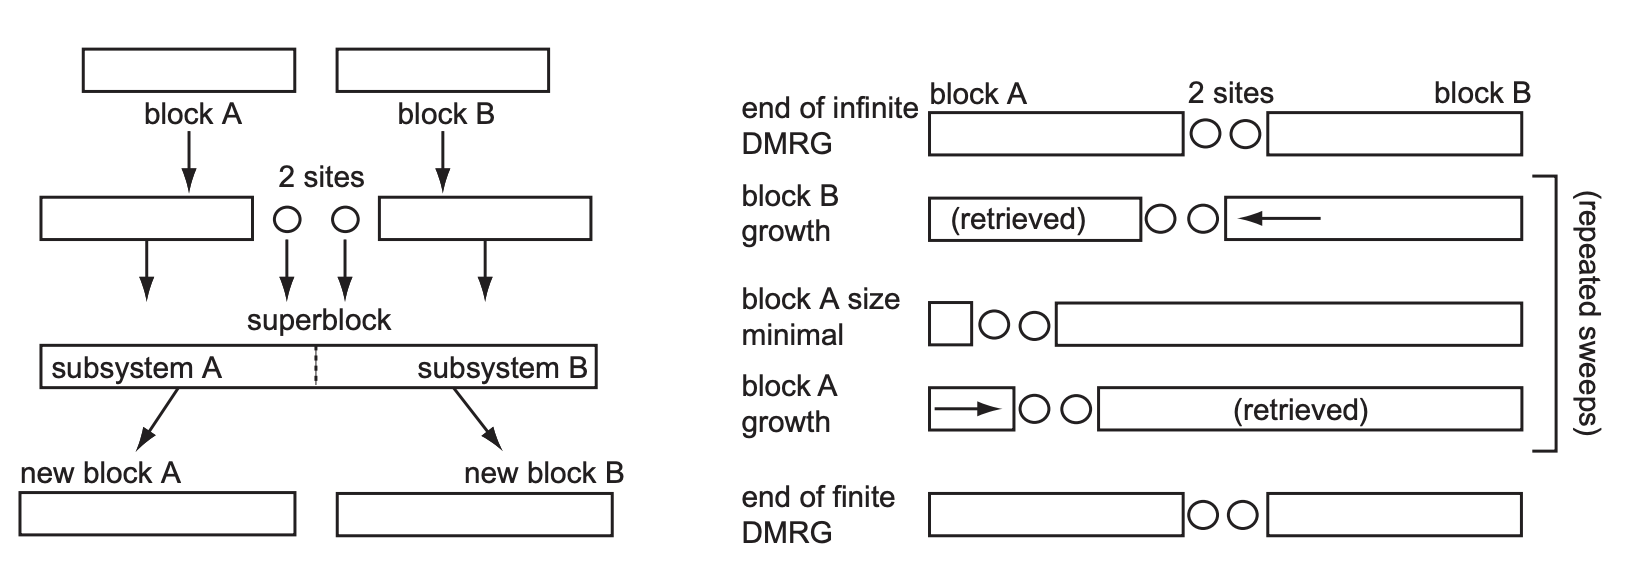
\includegraphics[width=0.70\linewidth]{figures/fig1.png}
    \caption{The left and right half the figure represent different iterations taken in the infinite system and finite system DMRG procedures respectively. In both cases, new blocks are formed from integrating a site into a block, with a state space truncation according to the density-matrix prescription of DMRG. Whereas in the infinite-system version this growth happens on both sides of the chain, leading to chain growth, in the finite-system algorithm it happens only for one side at the expense of the other, leading to constant chain length.}
    \label{fig:placeholder}
\end{figure}
\noindent We introduce left and right blocks A and B, which in a first step may consist of one spin (or site) each, such that total chain length is 2. Longer chains are now built iteratively from the left and right ends, by inserting pairs of spins between the blocks, such that the chain grows to length 4, 6, and so on; at each step, previous spins are absorbed into the left and right blocks, such that block sizes grow as 1, 2, 3, and so on, leading to exponential growth of the dimension of the full block state space as $2^l$ where $l$ is the current block size. The reduced block state space is of dimension D and say that for a block A of length $l$ it has D dimensional reduced Hilbert space with orthonormal basis $\{ \ket{a_l}_A\}$.

\vspace{1em}

\noindent We say that any state of the superblock is defined as the following where the states of the site next to A are in set $\{ \ket{\sigma}_A\}$ of local state space dimension $d$ (and same for those next to site B).

\[
\ket{ \psi } = \sum_{a_A \sigma_A \sigma_B a_B} \psi_{a_A \sigma_A \sigma_B a_B} 
\Ket{a}_A \Ket{\sigma}_A \Ket{\sigma}_B \Ket{a}_B 
\equiv \sum_{i_A j_B} \psi_{i_A j_B} \Ket{i}_A \Ket{j}_B
\]

\noindent Now we simply use some numerical sparse matrix eigen-solving technique such as \href{https://en.wikipedia.org/wiki/Lanczos_algorithm}{\emph{Lanczos}} to yield the respective wavefunction as most matrix elements are zero: 

\[
E= \frac{\Braket{\psi | \hat{H}_{A \bullet \bullet B} | \psi}}{\Braket{\psi | \psi}}
\]

\noindent Taking the states $\{ \ket{i}_A\}$ as the basis for left block: $A \bullet$ the dimension grows to $dD$, in order to truncate it back to D we define the reduced density operator for block $A \bullet$ where: 

\[
\hat{\rho}_{A_\bullet} = \mathrm{Tr}_{\bullet B} \Ket{\psi} \Bra{\psi} \qquad 
\left( \rho_{A_\bullet} \right)_{ii'} = \sum_j \psi_{ij} \psi^*_{i'j}
\]
\noindent In the decimation procedure we truncate by retaining as a reduced basis the D orthonormal eigenstates that have the largest associated eigenvalues: $w$. If they are called $\ket{b}_A$ the vector entries are the expansion coefficients in the previous block-site basis $_A\braket{a \sigma \mid b}_A$.

\vspace{1em}

\noindent There are two reasons for the truncation procedure:
\begin{itemize}
    \item We are interested in the states of $A\bullet$ contributing most of the ground state for $A\bullet$ embedded in the final, much larger (possibly infinite) system. 
    \item The prescription above follows from demanding that the 2-norm distance $\lVert \ket \psi - \ket \psi_{\text{trunc}} \rVert$ between the current ground state $\ket \psi$ and its projection onto the truncated black bases of dimension D, $\ket \psi_{\text{trunc}}$ is minimal. 
\end{itemize}

\noindent The overall success of DMRG rests on the fact that even for moderate D (often only a few 100) the total weight of the truncated eigenvalues has truncation error given by $\epsilon = 1 - \sum_{a > D} w_a$ if we assume descending order of the $w_a$ is small $\sim 10^{-10}$. The success of this algorithm is improved by exploiting quantum symmetries such as the $\mathbb{Z}_2$ mirror symmetry\footnote{The $\mathbb{Z}_2$ mirror symmetry is a discrete symmetry corresponding to reflection (left $\leftrightarrow$ right) of the system. In a spin chain, for instance, it means that the Hamiltonian is unchanged if the sites are reversed, i.e. $i \rightarrow N - i + 1$.}, additionally Abelian symmetries like the $U(1)$ symmetry of particle number ("charge") or magnetization conservation\footnote{The $U(1)$ symmetry corresponds to conservation of a continuous quantity such as total particle number or total magnetization. Physically, this means the Hamiltonian commutes with the number (or magnetization) operator, e.g. $[\hat{H}, \hat{N}] = 0$, and the wavefunction acquires only a phase under global rotations in that quantity’s space.} and non-Abelian symmetries like the $SU(2)$ symmetry of rotational invariance\footnote{The $SU(2)$ symmetry represents full spin rotational invariance: the Hamiltonian is unchanged under any spin rotation. This implies conservation of total spin, $\mathbf{S}^2$, and its components, allowing states to be grouped by total spin quantum number $S$.}.


\vspace{1em}

\noindent We can demonstrate the $U(1)$ symmetry associated with magnetization conservation. Assume the total magnetization $\hat M=\sum_i \hat S_i^{,z}$ commutes with the Hamiltonian, $[\hat H,\hat M]=0$, so energy eigenstates can be chosen to be eigenstates of $\hat M$. If we target the sector $M=0$ and choose block and site bases that are magnetization eigenstates, then a coefficient $\psi_{a_A\sigma_A\sigma_B a_B}$ can be nonzero only when $M(\ket a_A)+M(\ket \sigma_A)+M(\ket \sigma_B)+M(\ket a_B)=0$. This selection rule prunes all charge-mismatched entries, yielding a substantial speedup. Equivalently, writing the state as a matrix $\Psi$ with left indices $(a_A,\sigma_A)$ and right indices $(\sigma_B,a_B)$, the reduced density matrix $\rho_{A\bullet}=\mathrm{Tr}_{B\bullet}(\ket\psi\bra\psi)=\Psi\Psi^\dagger$ commutes with the left charge and is therefore block diagonal in magnetization sectors. Diagonalizing $\rho_{A\bullet}$ sector by sector and retaining the $D$ eigenvectors with the largest eigenvalues $w_a$ gives the optimal rank-$D$ truncation with truncation error. Thus symmetry both removes forbidden tensor blocks apriori and preserves quantum numbers during truncation.

\vspace{1em}

\noindent Lets now consider an operator $\hat O$ acting on site $l$ with matrix elements given as $O^{\sigma_l \sigma_l'} = \braket{\sigma_l \mid \hat O_l \mid \sigma_l'}$. Without loss of generality assume site $l$ is on left hand side and added into block A. As the block grows from $l-1 \rightarrow l$ as: 

\[
\braket{a_{\ell} | \hat{O} | a'_{\ell}} = \sum_{a_{\ell-1}, \sigma_{\ell}, \sigma'_{\ell}} 
\braket{a_{\ell} | a_{\ell-1} \sigma_{\ell}} 
\braket{\sigma_{\ell} | \hat{O} | \sigma'_{\ell}} 
\braket{a_{\ell-1} \sigma'_{\ell} | a'_{\ell}}.
\]

\noindent Where $\ket{a_l}$ and $\ket{a_{l-1}}$ are the effective basis states of blocks of length $l$ and $l-1$ respectively where realize that in the DMRG procedure the decimation process . As the block grows updates are made to the blocks as:

\begin{align*}
\braket{a_{\ell+1} | \hat{O} | a'_{\ell+1}} &= \sum_{a_{\ell} a'_{\ell} \sigma_{\ell+1}} 
\braket{a_{\ell+1} | a_{\ell} \sigma_{\ell+1}} 
\braket{a_{\ell} | \hat{O} | a'_{\ell}} 
\braket{a'_{\ell} \sigma_{\ell+1} | a'_{\ell+1}}\\
&= \sum_{a_{\ell} \sigma_{\ell+1}} 
\braket{a_{\ell+1} | a_{\ell} \sigma_{\ell+1}} 
\left( \sum_{a'_{\ell}} 
\braket{a_{\ell} | \hat{O} | a'_{\ell}} 
\braket{a'_{\ell} \sigma_{\ell+1} | a'_{\ell+1}} 
\right) 
\end{align*}

\noindent Note in hamiltonians when matrix products, $\hat{O}\hat{P}$ occur, due to the many truncation steps to insert the quantum mechanical one in the current block basis is highly imprecise. Rather the correct way is to update the first operator (counting from the left for a left block A) until the site of the second operator is reached, and to incorporate it as:

\begin{align*}
\braket{a_{\ell} | \hat{O} \hat{P} | a'_{\ell}} 
&\neq \sum_{\tilde{a}_{\ell}} 
\braket{a_{\ell} | \hat{O} | \tilde{a}_{\ell}} 
\braket{\tilde{a}_{\ell} | \hat{P} | a'_{\ell}} \text{\ding{55}} \\
&= \sum_{a_{\ell-1} a'_{\ell-1} \sigma_{\ell} \sigma'_{\ell}} 
\braket{a_{\ell} | a_{\ell-1} \sigma_{\ell}} 
\braket{a_{\ell-1} | \hat{O} | a'_{\ell-1}} 
\braket{\sigma_{\ell} | \hat{P} | \sigma'_{\ell}} 
\braket{a'_{\ell-1} \sigma'_{\ell} | a'_{\ell}} \text{\ding{51}}
\end{align*}

\noindent The final evaluation of expectation values is given at the end of the growth procedure as:

\begin{align*}
\braket{\psi | \hat{O} | \psi} = 
\sum_{a_A a'_A \sigma_A \sigma_B a_B} 
\braket{\psi | a_A \sigma_A \sigma_B a_B} 
\braket{a_A | \hat{O} | a'_A} 
\braket{a'_A \sigma_A \sigma_B a_B | \psi}
\end{align*} 

\noindent In the case of a anisotropic $S = \frac12$ Heisenberg antiferromagnetic $J = 1$ spin chain model where we assume the Zeeman magnetic field has zero effect, $h=0$ that the Hamiltonian can be represented as follows :

\[
 \hat H =\sum_{i=1}^{L-1} \frac{J}{2} \left( \hat{S}_i^+ \hat{S}_{i+1}^- + \hat{S}_i^- \hat{S}_{i+1}^+ \right) + J^z \hat{S}_i^z \hat{S}_{i+1}^z = \sum_{i=1}^{L-1} \sum_{\alpha=x,y,z} \hat{S}_i^\alpha \hat{S}_{i+1}^\alpha 
\]

\noindent In the DMRG procedure we represent the enlarged block Hamiltonian by:

\[
H_{A}^{(\ell+1)}
= {U^{[\ell+1]}}^{\!\dagger}\!\left(
  H_{A}^{(\ell)}\otimes I
  + J\sum_{\alpha=x,y,z}
    S_{A,\mathrm{edge}}^{\alpha(\ell)}\otimes S^{\alpha}
\right) U^{[\ell+1]} \qquad S_{A,\mathrm{edge}}^{\alpha(\ell+1)}
= {U^{[\ell+1]}}^{\!\dagger}\,\bigl(I_{A}^{(\ell)}\otimes S^{\alpha}\bigr)\,U^{[\ell+1]} 
\]

\noindent At the initialization step \(\ell=1\), we set \(H_A^{(1)}=\mathbf0\) and \(S_{A,\mathrm{edge}}^{\alpha\,(1)}=S^\alpha\). Here we represent the isometry $U^{[\ell+1]}$ as our coulums of the kept subspace from the decimation procedure where $U^{[\ell+1]\dagger}U^{[\ell+1]} = \mathbbm{1}$.

\subsection{Finite System DMRG (fDMRG)}\label{subsec:fdmrg}

\noindent Once the desired final system size is reached by infinite-system DMRG, it is important in all but the most trivial applications to follow up on it by the so-called finite-system DMRG procedure. This will not merely lead to some slight quantitative improvements of our results, but may change them completely. 

\vspace{1em}

\noindent The finite system case continues the growth process of, say without loss of generality block B, following the same prescription as before: finding the ground state of the superblock system, determining the reduced density operator, finding the eigensystem, retaining the D highest weight eigenstates for the next larger block. But it does so at the expense of block A, which shrinks (i.e. old shorter blocks A are reused). This is continued until A is so small as to have a complete Hilbert space, i.e. of dimension not exceeding D (one may also continue until A is merely one site long; results are not affected). Then the growth direction is reversed: A grows at the expense of B, including new ground state determinations and basis choices for A, until B is small enough to have a complete Hilbert space, which leads to yet another reversal of growth direction. 

\vspace{1em}

\noindent This sweeping through the system is continued until energy (or, more precisely, the wave function) converges. The intuitive motivation for this (in practice highly successful) procedure is that after each sweep, blocks A or B are determined in the presence of an ever improved embedding. 

\vspace{1em} 

\noindent In practice, this algorithm involves a lot of book-keeping, as all the operators we need have to be maintained in the current effective bases which will change from step to step thus truncated basis transformations determined have to be carried out after each step; operator representations in all bases have to be stored, as they will be needed again for the shrinking block. Another important feature is that for finding the ground state $\ket{\psi}$ for each $A\bullet\bullet B$ configuration one employs some iterative large sparse matrix eigen-solver based on sequential applications of $\hat{H}$ on some initial starting vector.

\subsection{Python Implementation}

\noindent The DMRG procedure can demonstrated used the Numerical Python Library and th. We first import the necessary library's and define the Pauli spin operators for a single site. 

\vspace{1em}

\begin{python}
import numpy as np
import scipy.sparse as sparse
from scipy.sparse import kron, eye , csr_matrix
from scipy.sparse.linalg import eigsh, eigs
from scipy.linalg import eigh
\end{python}

\begin{python}
d = 2 # "d" must be the on-site Hilbert-space dimension (e.g., d=2 for spin-1/2)
Sx = 0.5*np.array([[0, 1], [1, 0]], dtype=complex)
Sy = 0.5*np.array([[0, -1j], [1j, 0]])
Sz = 0.5*np.array([[1, 0], [0, -1]], dtype=complex)
Id = eye(d, dtype=complex, format='csr')
\end{python}

\vspace{1em}

\noindent We can define the \verb|Block| representing the left or right system block. Note that \verb|S_edge| contains the spin operators on the right edge of the block since it tells us how the block interacts with the environment after the original block has been transformed into a new basis during the renormalization process.

\vspace{1em}

\begin{python}
class Block:
    """ Renormalized block for two - site DMRG (sparse implementation)"""
    def __init__ (self, dim: int, 
                  H: csr_matrix, # Sparse Hamiltonian
                  S_edge: tuple [ csr_matrix , csr_matrix , csr_matrix ]): # Sparse operators 
        self.dim = dim # Hilbert space dimension
        self.H = H # Block Hamiltonian (sparse)
        self.S_edge = S_edge # Tuple of (Sx , Sy , Sz) on RIGHT edge (sparse)
\end{python}

\vspace{1em}

\noindent Next, we define the function that enlarges the block by adding one site and truncating to $m_{\text{keep}}$ states. To demonstrate the process, we first assume we have obtained a block of $n$ sites and we want to add an additional site $n+1$. The dimension of the Hamiltonian is $m = \dim(Hn) = \min\{m_{\text{keep}}, 2n\}$, where $m_{\text{keep}}$ is the number of states we want to keep after truncation.

\vspace{1em}

\noindent For the DMRG process there are a total of six steps that are implemented which follow the procedure outlined above. The \verb|englarge_block| function takes in an instance of a Block and the number of states to keep in the truncation procedure $m_{\text{keep}}$. 

\begin{enumerate}
    \item Initially we start the Hamiltonian on the enlarged space then add the edge–site interaction terms:
        \[H_{\text{left}} = H_{\text{block}} \otimes I_d + \sum_{\alpha=x,y,z} S_i^\alpha S_{i}^\alpha\]
    \item Following that we create the environment block which is a mirror image of the left block 
        \[H_{\text{right}} = I_d  \otimes H_{\text{block}} + \sum_{\alpha=x,y,z} S_i^\alpha S_{i}^\alpha\]
    \item From there we can create the superblock Hamiltonian as:
        \[ H_{\mathrm{super}} = H_{\text{left}}\otimes I_{2m} + I_{2m}\otimes H_{\text{right}} + \sum_{\alpha=x,y,z}  S_{L}^{\alpha}\otimes S_{R}^{\alpha}\]
    \item Then we find the ground state wavefunction $\Psi$ of the superblock Hamiltonian through a sparse eigen-solver 
    \item Using the ground state wavefunction calculated previously we can compute the reduced density matrix and diagonalize it: 
        \[\rho = \Psi \Psi^{\dagger} \qquad \rho = U D U^{-1} \qquad U \xrightarrow{\text{truncate}} U_{\text{tr}} \]
    \item Finally comes the projection procedure where the operators are imposed onto the reduced basis created from the $m_{\text{keep}}$ largest eigenvectors of $U$. 
        \[ H_{\text{new}} = U_{\mathrm{tr}}^{\dagger}\,H_{\text{left}}\,U_{\mathrm{tr}}, \qquad S_{\text{new}}^{\,\alpha} = U_{\mathrm{tr}}^{\dagger}\,S_{R}^{\,\alpha}\,U_{\mathrm{tr}} \]
\end{enumerate}

\vspace{1em}

\begin{python}
    def englarge_block(block: Block, m_keep: int) -> tuple[Block, float]:
        """
        Add one site to block and truncate to m_keep states using sparse matrices. 
        Returns newblock and ground state energy of 4 - site superblock.
        """
    
        m, d = block.dim, 2

        # (1) Build extended left block (block + new site)
        # Hamiltonian : H_block I + interactions between block edge and new site
        H_left = kron(block.H, Id, format='csr')
        for Sb, Ss in zip(block.S_edge, (Sx, Sy, Sz)):
            H_left += kron(Sb, Ss, format='csr')

        # New right - edge operators (acting on the new site)
        I_m = eye(m, format='csr')
        Sx_R = kron(I_m, Sx, format='csr')
        Sy_R = kron(I_m, Sy, format='csr')
        Sz_R = kron(I_m, Sz, format='csr')
        left_block = Block(m * d, H_left, (Sx_R, Sy_R, Sz_R))

        # (2) Build environment block (mirror of left block)
        # For reflection symmetry , environment uses same operators as left block
        env_block = left_block
        mL, mR = left_block.dim, env_block.dim # mL = mR = 2 * m
        I_L = eye(mL, format='csr')
        I_R = eye(mR, format='csr')

        # (3) Construct 4 - site superblock Hamiltonian    
        H_super = kron(left_block.H, I_R, format='csr') # Left block Hamiltonian
        H_super += kron(I_L, env_block.H, format='csr') # Environment Hamiltonian

        # Coupling between left - block ’s right edge and environment ’s left edge
        for SL, SR in zip(left_block.S_edge, env_block.S_edge):
            H_super += kron(SL, SR, format='csr')

        # (4) Find superblock ground state
        Evals, Psi = eigsh(H_super, k=1, which='SA')
        E0, psi0 = Evals[0], Psi[:, 0]

        # (5) Compute reduced density matrix
        # Reshape wavefunction to bipartite form and compute density matrix
        psi_mat = psi0.reshape(mL, mR)
        rho = psi_mat @ psi_mat.conj().T
        rho = (rho + rho.conj().T)/2 # Ensure Hermiticity

        # Diagonalize density matrix and keep largest m_keep eigenvectors
        n_keep = min(m_keep, mL)
        evals, U = np.linalg.eigh(rho) # Dense diagonalization (small matrix)
        idx = np.argsort(evals)[::-1][:n_keep] # Descending order
        Utr = U[:, idx]

        # (6) Project operators into truncated basis
        # Convert to dense for efficient small matrix operations
        Utr_dense = Utr
        H_left_dense = H_left.toarray()
        Sx_R_dense = Sx_R.toarray()
        Sy_R_dense = Sy_R.toarray()
        Sz_R_dense = Sz_R.toarray()

        # Perform projections ( dense matrix multiplication )
        H_new = Utr_dense.conj().T @ H_left_dense @ Utr_dense
        Sx_new = Utr_dense.conj().T @ Sx_R_dense @ Utr_dense
        Sy_new = Utr_dense.conj().T @ Sy_R_dense @ Utr_dense
        Sz_new = Utr_dense.conj().T @ Sz_R_dense @ Utr_dense

        # Convert results back to sparse format
        H_new = csr_matrix(H_new)
        Sx_new = csr_matrix(Sx_new)
        Sy_new = csr_matrix(Sy_new)
        Sz_new = csr_matrix(Sz_new)
    
        return Block(n_keep, H_new, (Sx_new, Sy_new, Sz_new)), E0
\end{python}

\vspace{1em}

\noindent With the block growth procedure defined we can implement the Infinite DMRG algorithm; the iDMRG algorithm is implemented for systems at the thermodynamic limit, however we are able to get a good approximation by returning the ground state after every iteration. From above, the initial block is a single site with a sparse Hamiltonian: 

\[ H_{\mathrm{init}}=H_{1}= \begin{pmatrix} 0 & 0\\ 0 & 0 \end{pmatrix}, 
\qquad S_{\mathrm{edge}}^{\alpha}=(S_x,S_y,S_z). 
\]

\vspace{1em}

\begin{python}
    def infinite_dmrg(L_target: int, m_keep: int) -> tuple(list[Block], list[Block], float)
        """
        Iterativly run iDMRG algorithm for increasing larger spin chains L = 2, 4 ...
        """
            
        if L_target % 2:
            raise ValueError("L_target must be even")
    
        H_init = csr_matrix((d, d), dtype=complex) 
        block = Block(d, H_init, (Sx, Sy, Sz)) 
        groundstate_energies = []
    
        for L in range(2, int(L_target/2) + 1):
            block, E0 = englarge_block(block, m_keep) # solve ground state and truncate; returns new block and E0(superblock)
    
            total_sites = 2 * L # superblock size = left (L) + mirrored right (L)
            Esite = E0 / total_sites
    
            groundstate_energies.append(Esite)               
            print(f"Superblock size = {total_sites:>3d}, E ={E0:.12f}, E/site = {Esite:.12f}")
    
        return groundstate_energies[-1]
\end{python}

\vspace{1em}

\begin{python}
    # Run DMRG calculation
    energies = infinite_dmrg(L_target = 20, m_keep=24)
    print("Final energy density: ", energies[-1])
\end{python}

\vspace{1em}

\noindent To implement the finite DMRG algorithm we recall that we start with the iDMRG procedure and store the normalized blocks of length 1 to $L$ and store them as:

\begin{itemize}
    \item \verb|left_block| consisting of blocks of length: $1$, ..., $L$
    \item \verb|right_block| consisting of blocks of length $L$, ..., $1$
\end{itemize}

\noindent We perform first the sweep going left to right

\vspace{1em}

\begin{python}

\end{python}

\subsection{Python Implementation via Tensor Network Python Library}

\noindent The Tensor Network Python Library is a Python library for the simulation of strongly correlated quantum systems with tensor networks. These notes follow arXiv:2408.02010. 

\vspace{1em}

\noindent We import the Tensor Network Python Library and suppress any warning arising.   

\begin{python}
import warnings
from tenpy.models.spins import SpinChain
from tenpy.networks.mps import MPS
from tenpy.algorithms import dmrg

warnings.filterwarnings('ignore')
\end{python}

\vspace{1em}

\noindent To implement the system we use the different 

\vspace{1em}

\begin{python}
def ground_state_energy_spinchain(L, m_keep=16, sweeps=12):
    """
    Build a spin-1/2 isotropic Heisenberg (XXX) chain of length L with open boundaries
    """
    model_params = dict(
        L=L,                     # number of sites
        S=0.5,                   # on-site spin = 1/2
        Jx=1.0, Jy=1.0, Jz=1.0,  # isotropic couplings: J=1 in x,y,z
        hz=0.0,                  # no longitudinal magnetic field (h = 0)
        bc_MPS="finite"          # finite MPS => finite-DMRG on an open chain
    )
    
    M = SpinChain(model_params) # instantiate the TenPy model (builds the MPO and lattice)

    prod = (['up', 'down'] * ((L + 1) // 2))[:L] # Creates ["up", "down", ...] pattern
    psi = MPS.from_product_state(M.lat.mps_sites(), prod, bc=M.lat.bc_MPS) # makes initial MPS

    dmrg_params = {
        "trunc_params": {        # SVD truncation:
            "chi_max": m_keep,   # cap bond dim at m_keep
            "svd_min": 0.0       # avoid dropping singular values by magnitude cutoff 
        },  
        "mixer": True,           # add noise/mixer to escape local minima at low chi
        "max_sweeps": sweeps,    # number of left right sweeps
        "verbose": 1,            # print basic progress
    }

    if L <= 2:
        dmrg_params["active_sites"] = 1 # use 1-site DMRG for tiny chains to avoid scheduler assertion

    info = dmrg.run(psi, M, dmrg_params) # run finite DMRG
    return float(info["E"])
\end{python}

\vspace{1em} Running the 

\begin{python}

\end{python}

\subsection{Comparison with True Groundstate Energy}

We can compare the ground-state energies calculated with TenPy and NumPy with the values calculated using the exact diagonalization methods. The code is given below: 

\begin{python}
    def op_on_site(op, i, L, Id=np.eye(2)):
        mats = [Id]*L
        mats[i] = op
        out = mats[0]
        for m in mats[1:]:
            out = np.kron(out, m)
        return out
\end{python}

\begin{python}
    def heisenberg_chain(L, J=1.0, open_boundary=True, pauli_convention=True):
        if L < 2:
            raise ValueError("L must be >= 2")

        pref = J/4.0 if pauli_convention else J
    
        H = np.zeros((2**L, 2**L), dtype=complex)
        bonds = [(i, i+1) for i in range(L-1)]
        if not open_boundary:
            bonds.append((L-1, 0)) 
    
        for i, j in bonds:
            Sx_i = op_on_site(sx, i, L); Sx_j = op_on_site(Sx, j, L)
            Sy_i = op_on_site(sy, i, L); Sy_j = op_on_site(Sy, j, L)
            Sz_i = op_on_site(sz, i, L); Sz_j = op_on_site(Sz, j, L)
            H += pref * (Sx_i @ Sx_j + Sy_i @ Sy_j + Sz_i @ Sz_j)
    
        H = 0.5 * (H + H.conj().T)
        return H
\end{python}

\begin{python}
    def ground_state(H):
        evals, evecs = np.linalg.eigh(H)
        E0 = float(np.real(evals[0]))
        psi0 = evecs[:, 0]
        psi0 = psi0 / np.linalg.norm(psi0)
        return E0, psi0
\end{python}

\begin{python}
    L = 8                  
    J = 1.0
    open_boundary = True
    use_pauli_convention = True  
    
    H = heisenberg_chain(L, J=J, open_boundary=open_boundary,
                         pauli_convention=use_pauli_convention)
    E0, psi0 = ground_state(H)
    print(f"L = {L}, dim = {H.shape[0]}")
    print(f"Ground-state energy E0 = {E0:.10f}")
    print(f"Energy per site E0/L = {E0/L:.10f}")
\end{python}

\noindent Compairing the results of the 

\begin{center}
\renewcommand{\arraystretch}{1.15}
\begin{tabular}{|p{0.75cm}|p{2.5cm}|p{1.5cm}|p{1.5cm}|p{3.2cm}|p{3.2cm}|}
 \hline
 \multicolumn{6}{|c|}{Ground-state Energy Comparison ($m_{\text{keep}}=16$)}\\
 \hline
 Sites & Diagonalization & iDMRG & fDMRG & iDMRG with TenPy & fDMRG with TenPy \\
 \hline
 2  & 0 & 0 & 0 & 0 & 0 \\
 4  & 0 & 0 & 0 & 0 & 0 \\
 16 & 0 & 0 & 0 & 0 & 0 \\
 20 & 0 & 0 & 0 & 0 & 0 \\
 24 & 0 & 0 & 0 & 0 & 0 \\
 28 & 0 & 0 & 0 & 0 & 0 \\
 32 & 0 & 0 & 0 & 0 & 0 \\
 36 & 0 & 0 & 0 & 0 & 0 \\
 40 & 0 & 0 & 0 & 0 & 0 \\
 \hline
\end{tabular}
\end{center}

\subsection{Subspace Expansion}

\noindent Theses notes are taken from Phys. Rev. B 91, 155115. To be continued....

\end{document}